\setchapterstyle{kao}
\setchapterpreamble[u]{\margintoc}

\chapter{Beyond the Standard Model Neutrinos}
\labch{bsm_neutrinos}


\section{Neutrino Oscillations}

\subsection{Vacuum Oscillations}

\subsection{Oscillations in Matter}

% \subsection{Three-Flavor Oscillations}

\subsection{Atmospheric Neutrino Oscillations}

\subsubsection{Neutrino Production in the Atmosphere}

\subsubsection{Oscillations of Atmospheric Neutrinos}

\subsubsection{Matter Effects}

% \subsection{Solar neutrinos}
% \subsection{Reactor neutrinos}
% \subsection{Accelerator neutrinos}
% \subsection{Anomalies in Neutrino Oscillation Measurements}


\section{Heavy Neutral Leptons}

\subsection{Motivation for Heavy Sterile Neutrinos}

\subsection{Extending the Standard Model}

% taken from technote
% \begin{figure}[h]
%     \subfloat[\labfig{hnl_decay_modes_log_branching_ratio}]{
%         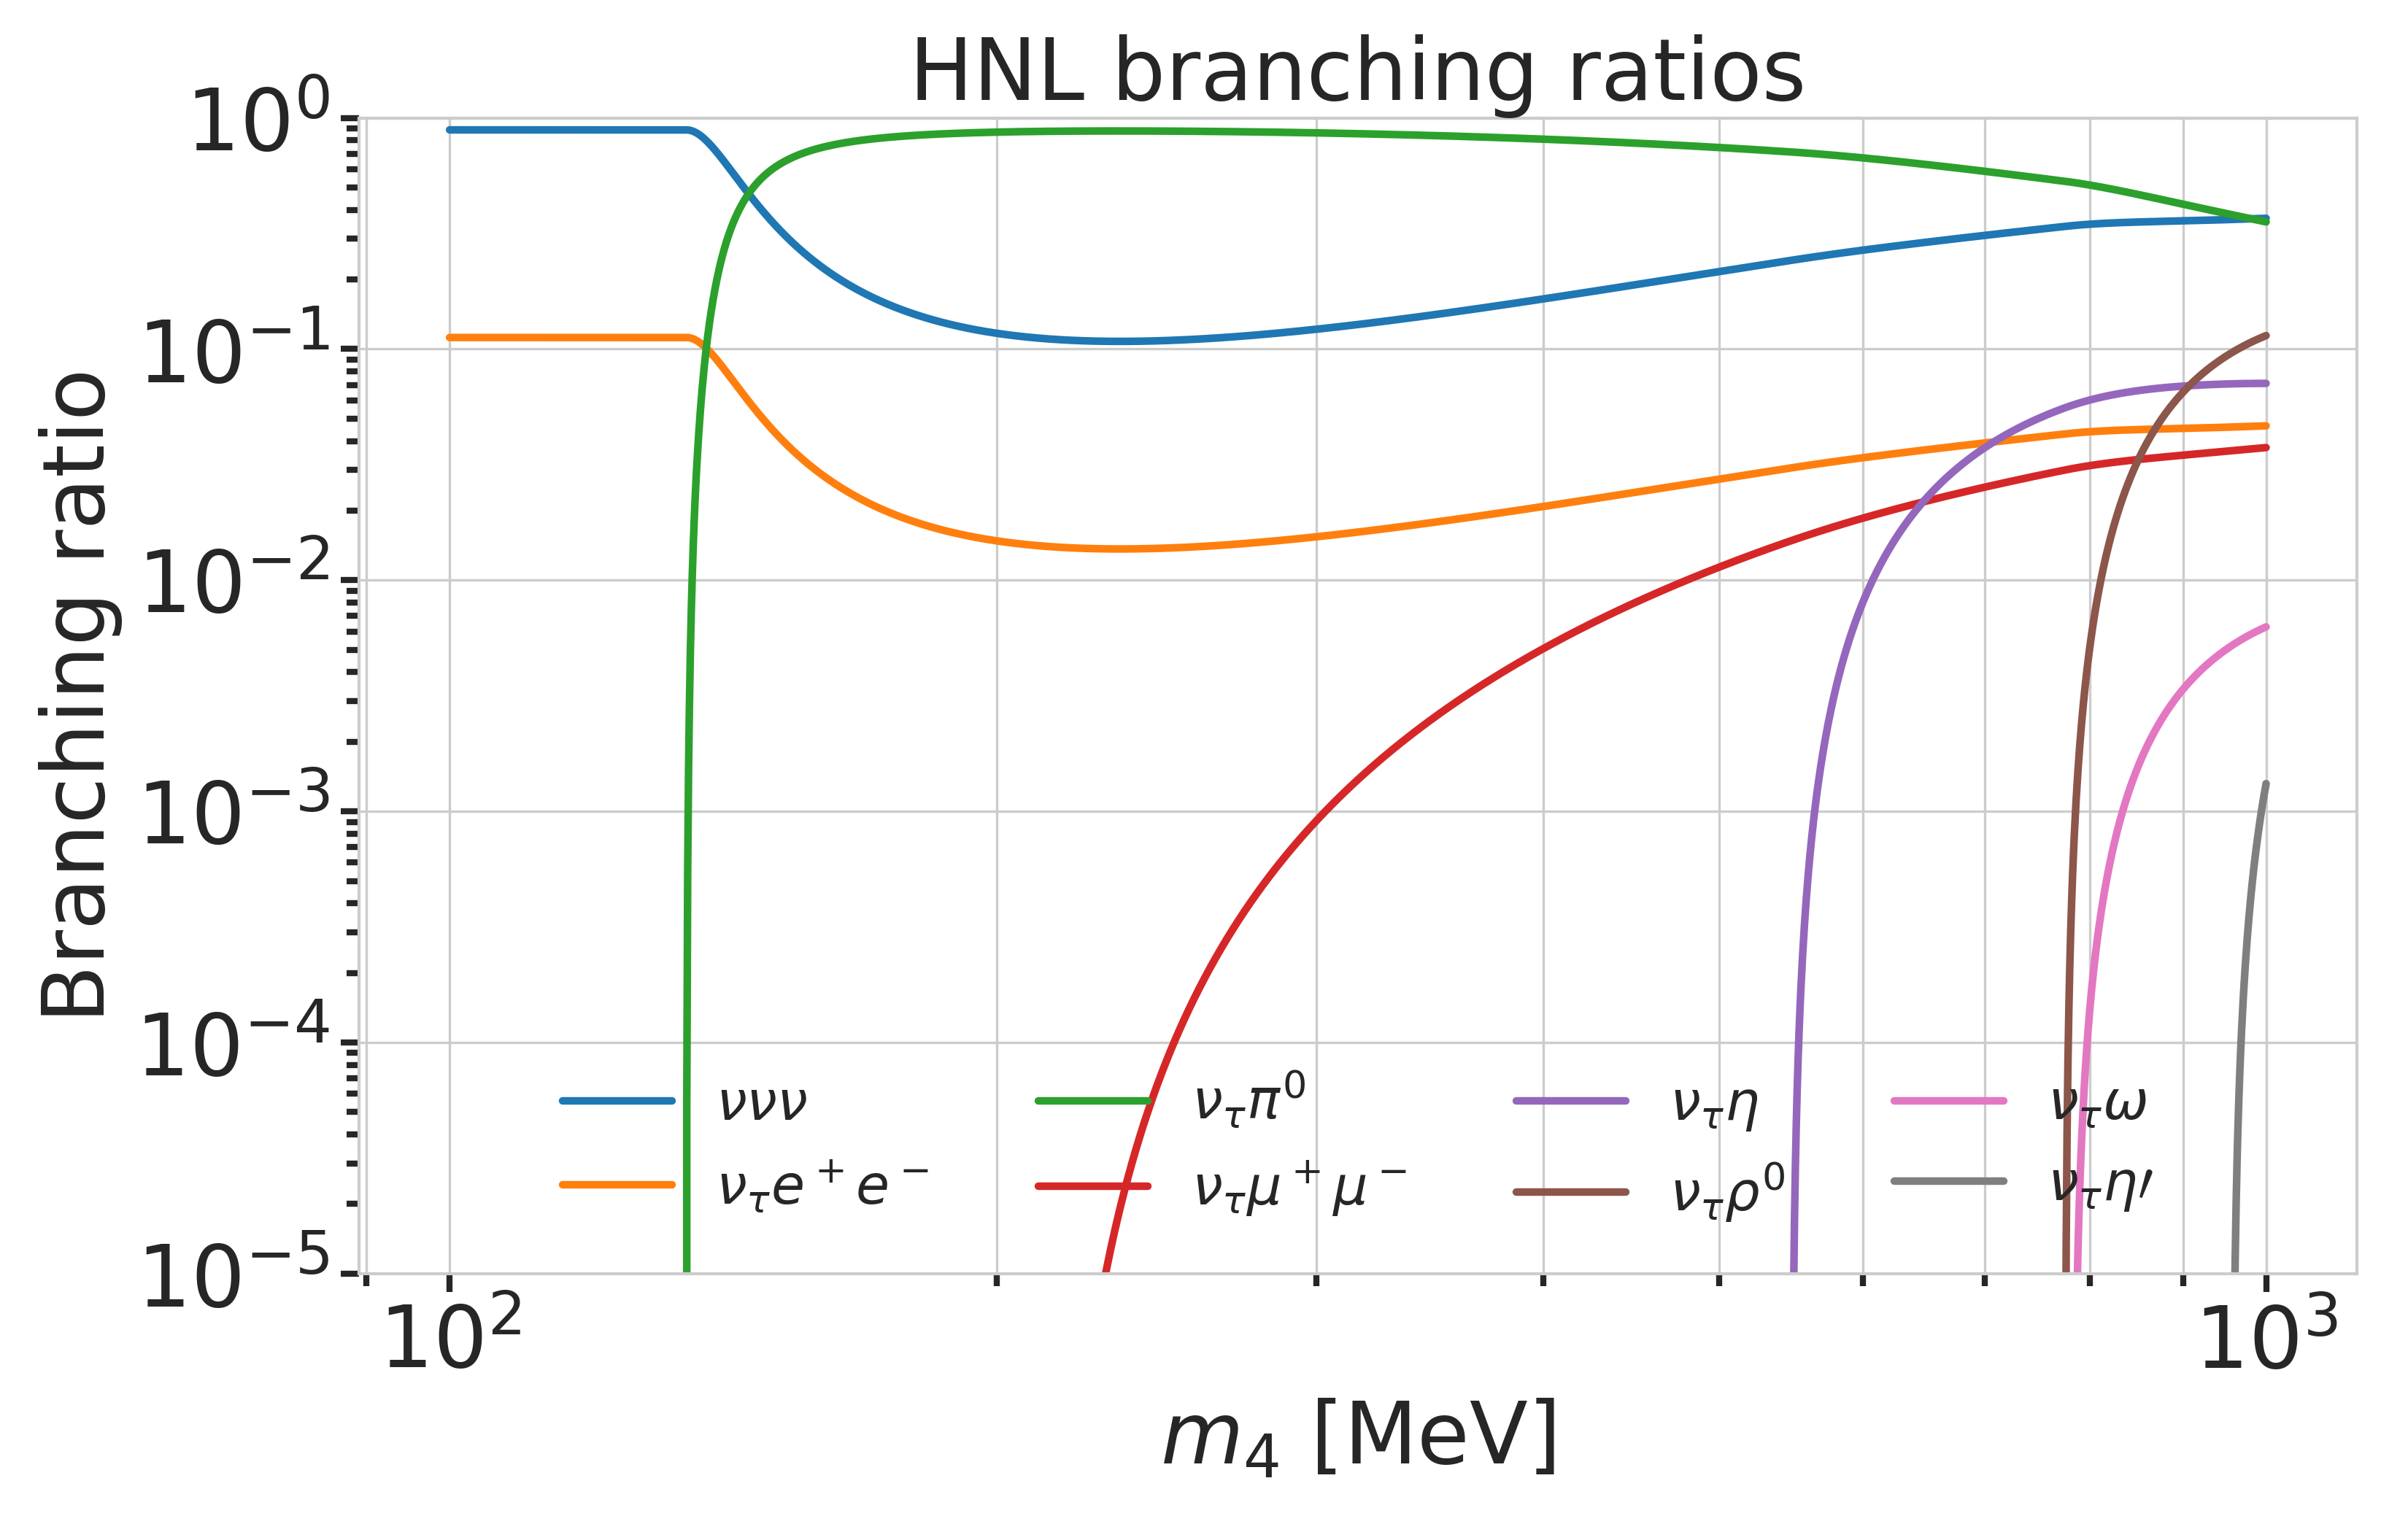
\includegraphics[width=.45\linewidth]{hnl_simulation/decay_theory/branching_ratios_log_up_to_1.0_GeV.png}
%     }
%     \subfloat[\labfig{hnl_decay_modes_log_decay_width}]{
%         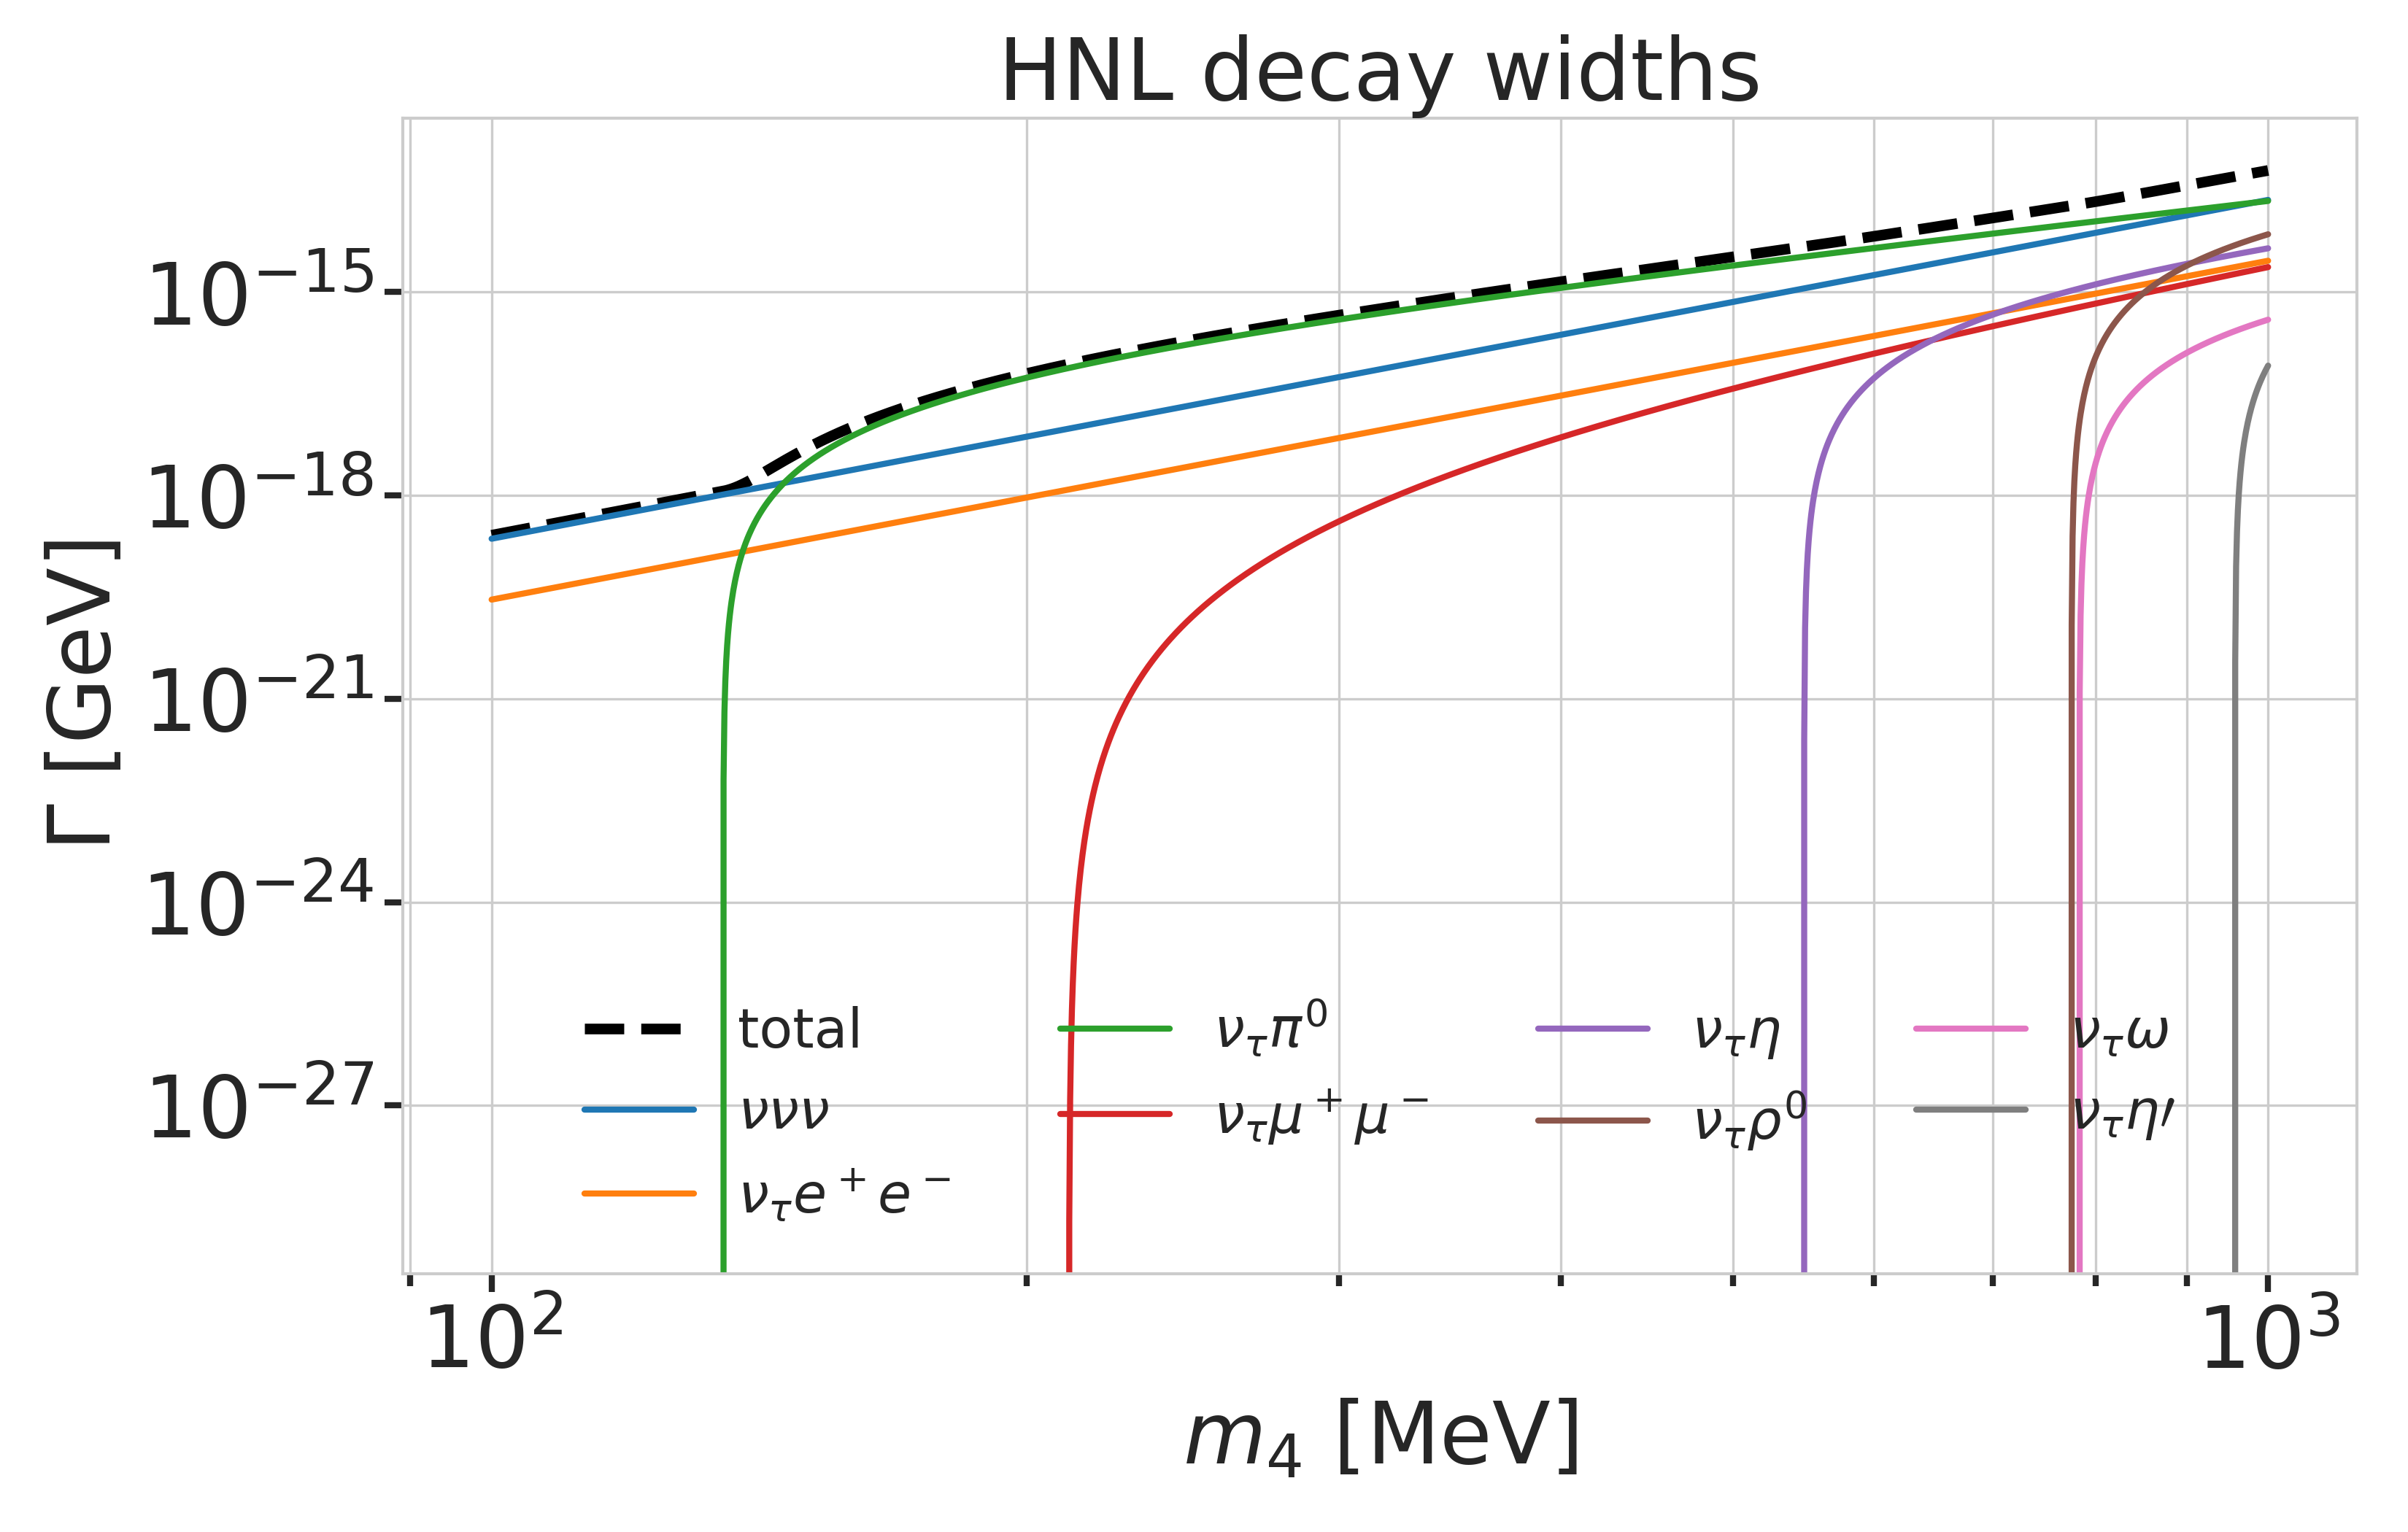
\includegraphics[width=.45\linewidth]{hnl_simulation/decay_theory/hnl_decay_widths_up_to_1.0_GeV_log.png}
%     }
%     \\[-2.5ex]
%     \centering
%     \subfloat[\labfig{hnl_decay_modes_log_proper_lifetime}]{
%         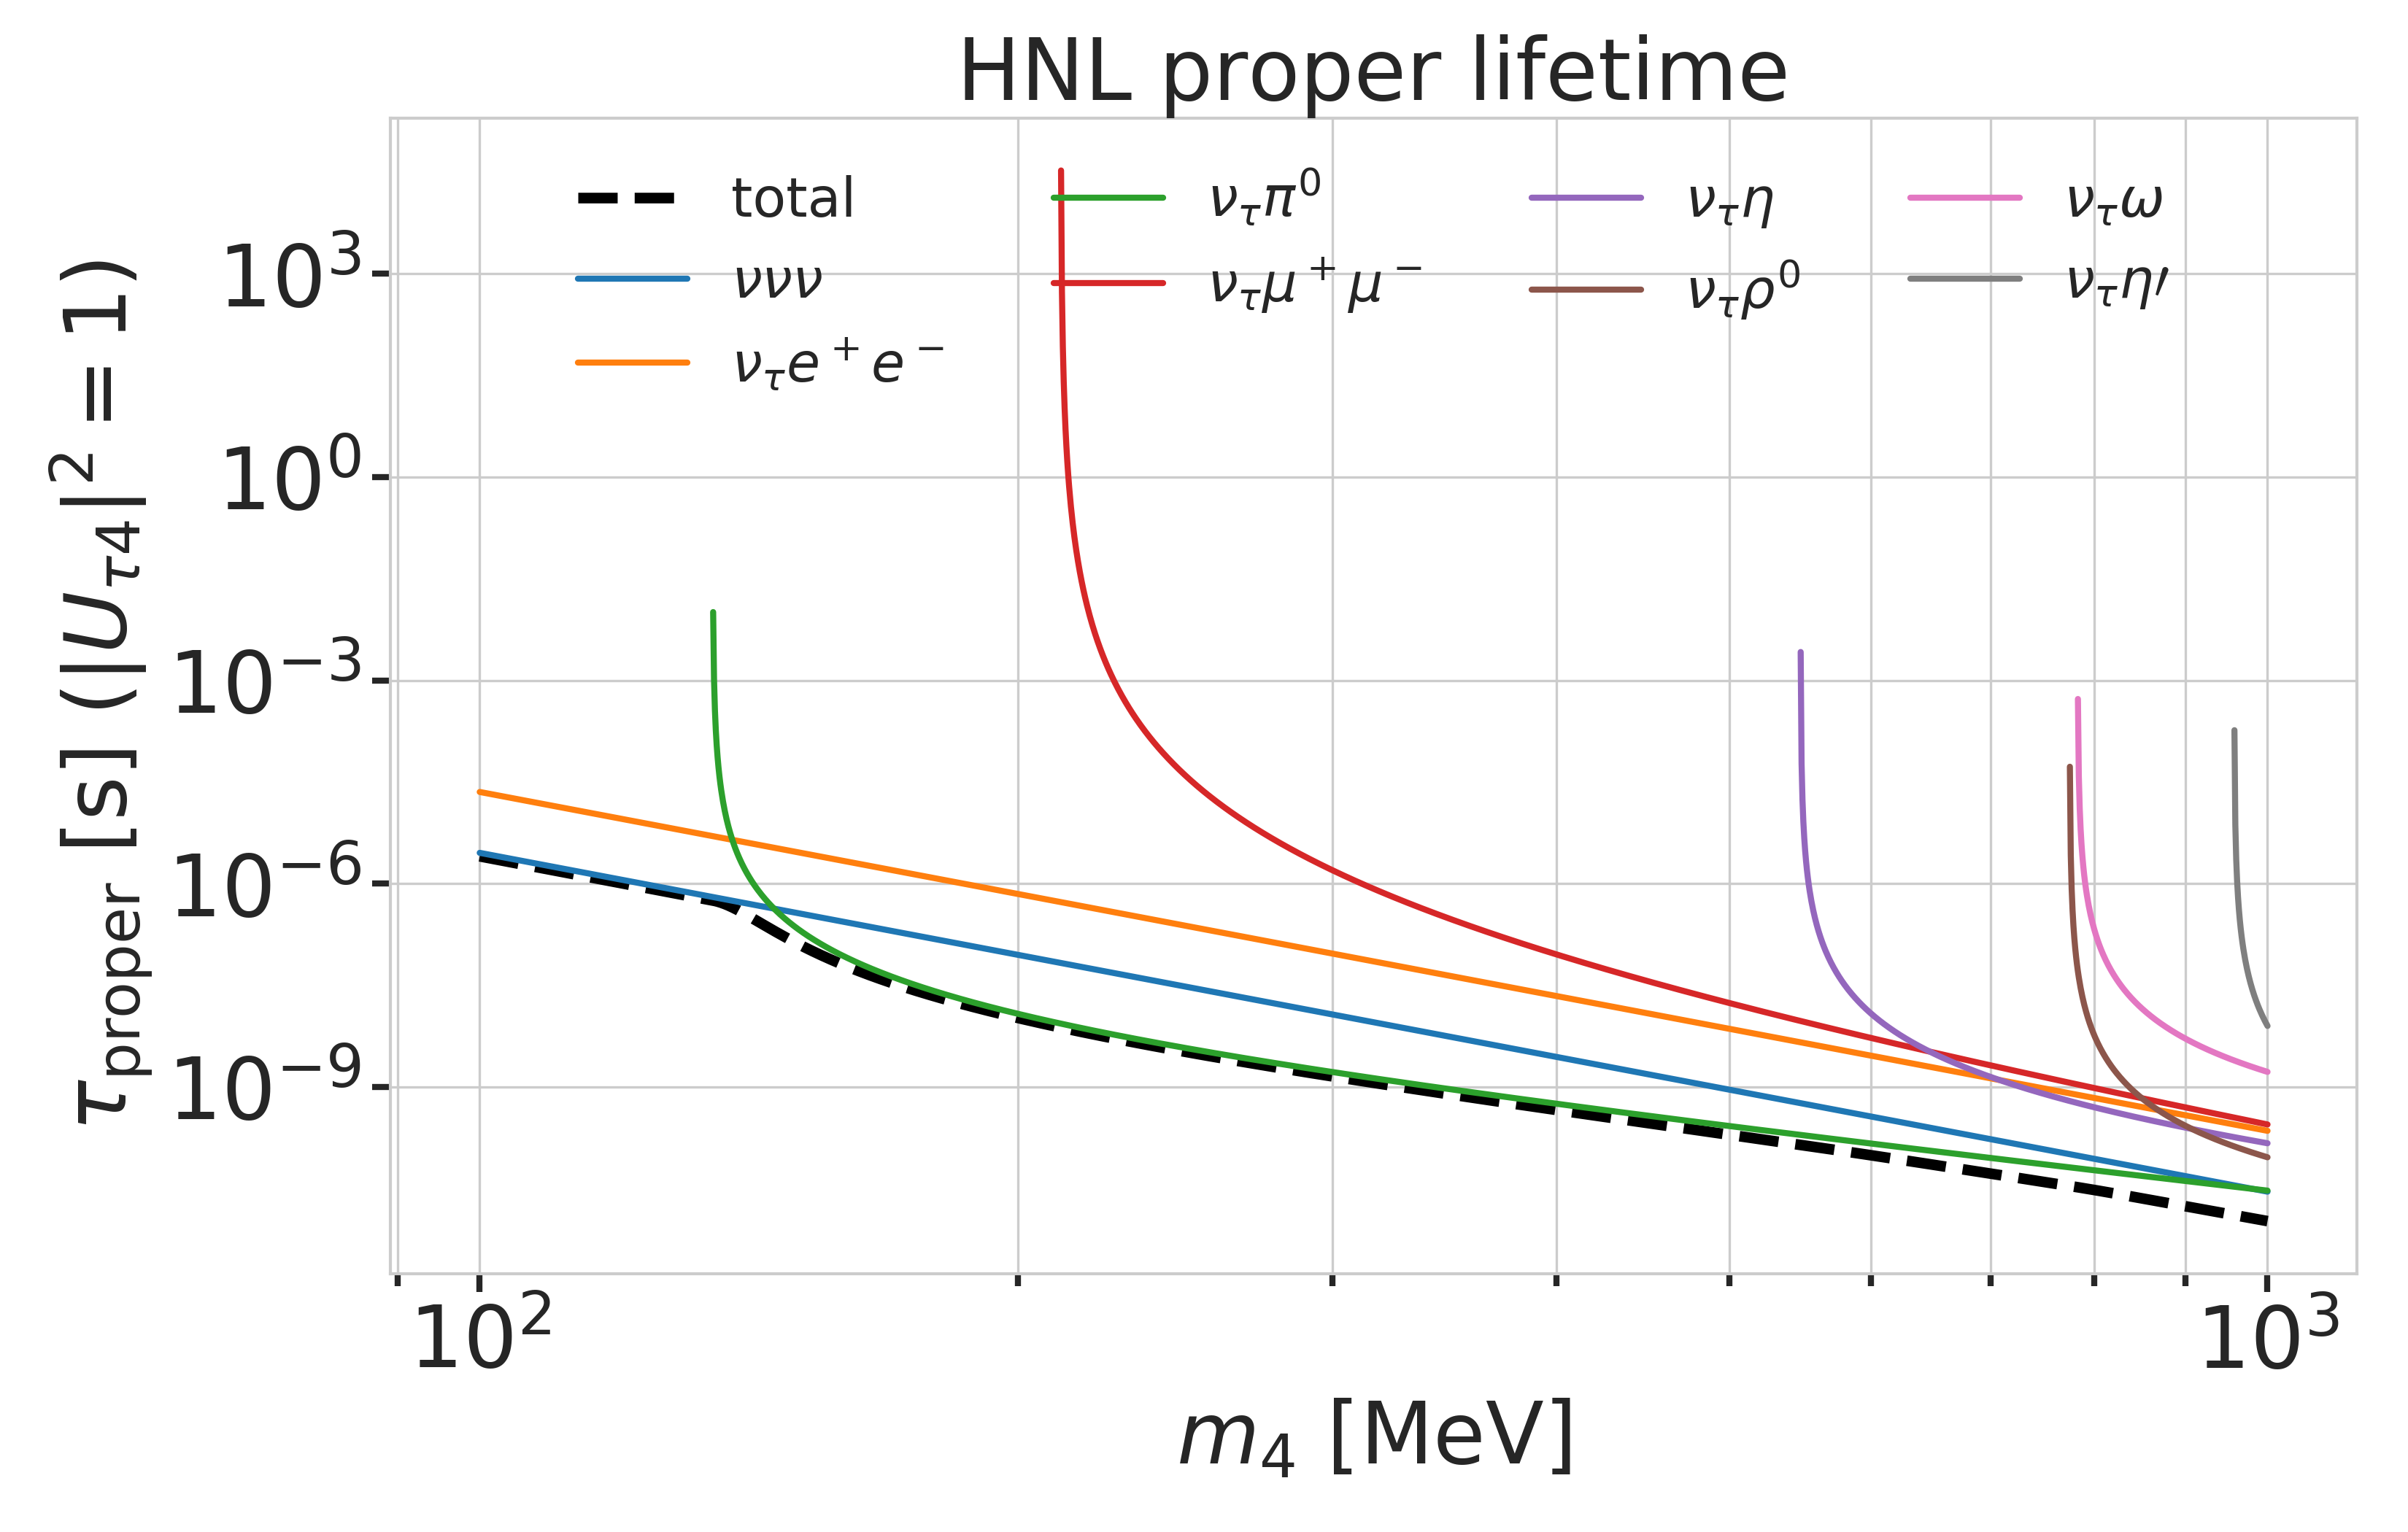
\includegraphics[width=.45\linewidth]{hnl_simulation/decay_theory/proper_lifetimes_up_to_1.0_GeV_log.png}
%     }
%     \caption{Branching ratios, decay widths, and proper lifetime of the HNL within the mass range considered, calculated based on the results from \sidecite{Coloma:2020lgy}. Given the existing constraints on $|U_{e4}|^{2}$ and $|U_{\mu4}|^{2}$, we consider that the corresponding decay modes are negligible.}
%     \labfig{hnl_decay_modes_log}
% \end{figure}

\begin{figure}
    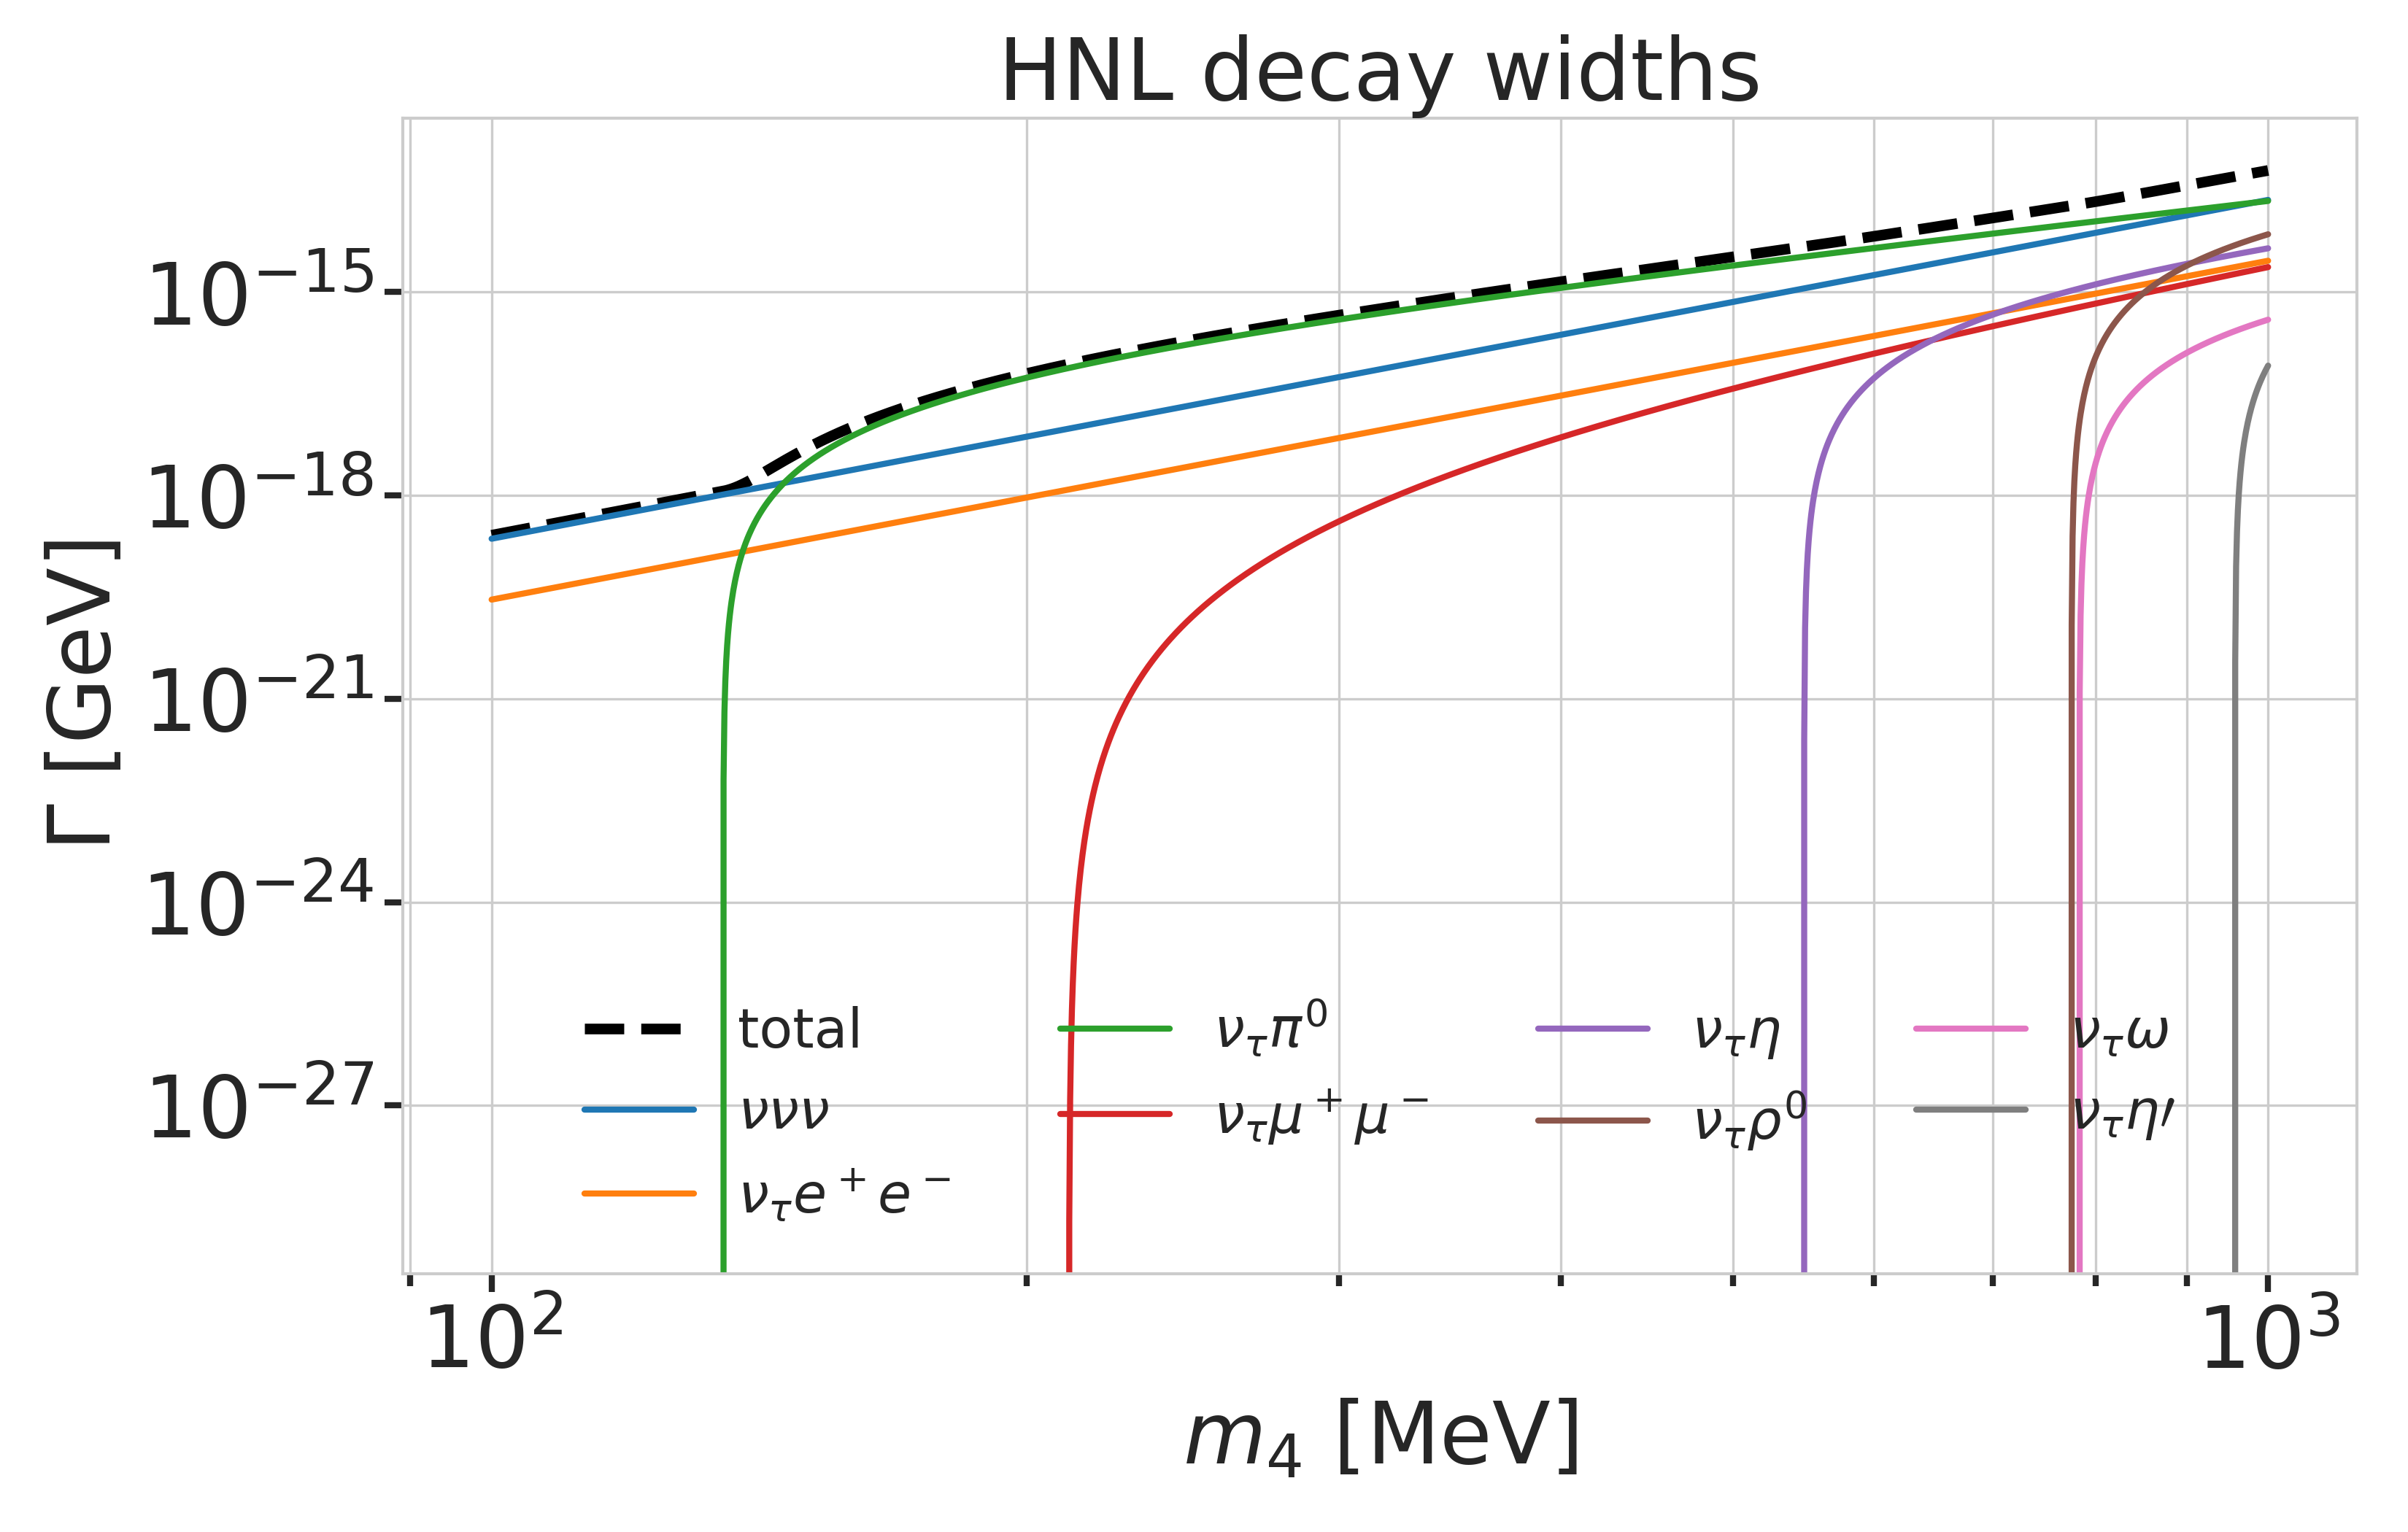
\includegraphics{hnl_simulation/decay_theory/hnl_decay_widths_up_to_1.0_GeV_log.png}
    \caption{Decay widths of the HNL within the mass range considered, calculated based on the results from \cite{Coloma:2020lgy}. Given the existing constraints on $|U_{e4}|^{2}$ and $|U_{\mu4}|^{2}$, we consider that the corresponding decay modes are negligible.}
    \labfig{hnl_decay_modes_log_decay_width}
\end{figure}


\subsection{Global Constraints on  mixing}


\section{Open Questions in Neutrino Particle Physics}
